\documentclass[border=10pt]{standalone}
\usepackage{tikz}\usepackage{amsmath}\usetikzlibrary{arrows.meta,patterns}
\begin{document}
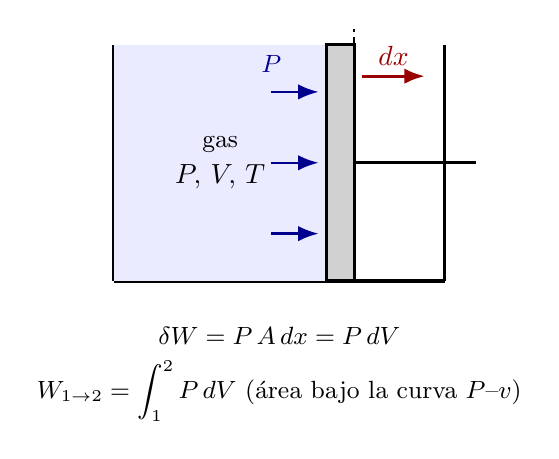
\begin{tikzpicture}[line width=0.9pt,>={Latex[length=2.6mm]}]
  % cilindro
  \draw[line width=1.2pt] (0,0)--(0,3) (4.2,0)--(4.2,3) (0,0)--(4.2,0);
  % gas
  \fill[blue!8] (0,0) rectangle (2.7,3);
  \node[align=center] at (1.35,1.5){\small gas\\[1pt]$P,\,V,\,T$};
  % piston
  \fill[black!18] (2.7,0) rectangle (3.05,3);
  \draw[line width=1.1pt] (2.7,0) rectangle (3.05,3);
  \draw[line width=1.1pt] (3.05,1.5)--(4.6,1.5);
  % presion del gas sobre el piston
  \foreach \y in {0.6,1.5,2.4} \draw[->,blue!55!black] (2.0,\y)--(2.6,\y);
  \node[blue!55!black] at (2.0,2.75){\small $P$};
  % desplazamiento
  \draw[->,red!60!black,line width=1.2pt] (3.15,2.6)--(3.95,2.6) node[midway,above]{$dx$};
  \draw[densely dashed] (3.05,0)--(3.05,3.2);
  \node at (2.1,-0.7){\small $\delta W=P\,A\,dx=P\,dV$};
  \node at (2.1,-1.4){\small $W_{1\to2}=\displaystyle\int_1^2 P\,dV$ (área bajo la curva $P$–$v$)};
\end{tikzpicture}
\end{document}
